\chapter{Mappa dell'India centro-orientale}

\vspace*{\baselineskip}

{\centering
  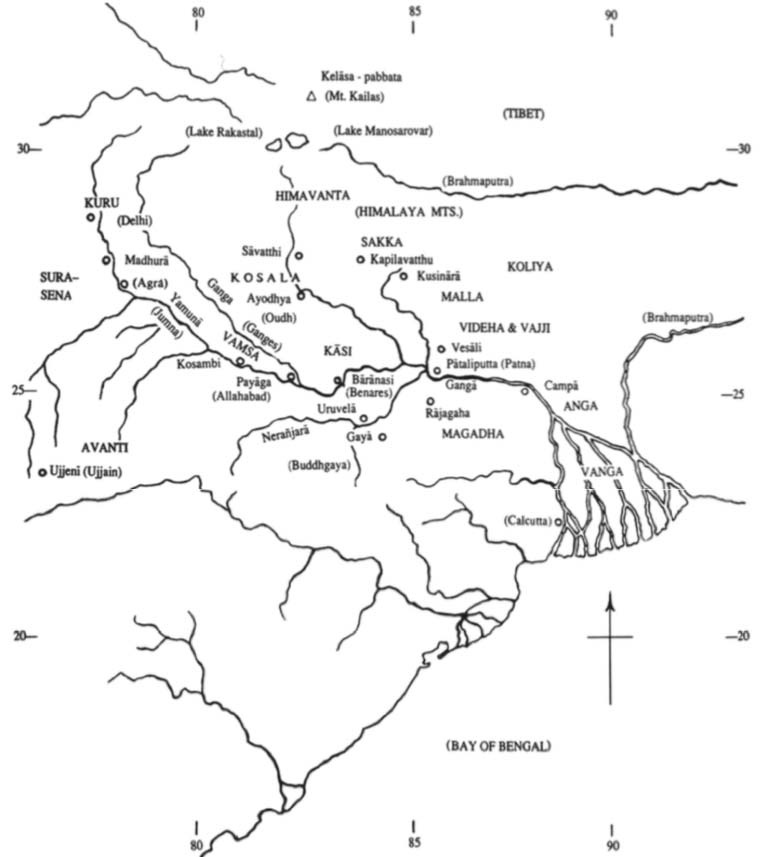
\includegraphics[width=\linewidth]{mappa.jpg}
\par}

\vspace*{1.5\baselineskip}

La mappa — tratta dalla \emph{Cambridge History of India, I: Ancient India}, ed.
by E.J. R Apson, Cambridge 1922, Map. 5 — mostra alcuni dei principali nomi
di luogo menzionati nel Canone in lingua pāli. I nomi moderni sono
racchiusi tra parentesi tonde.

